\section{BreastScreening}
\label{sec:sec004}
To validate the proposed design goals, we created \href{https://breastscreening.github.io/}{{\it BreastScreening}}, as a Medical Imaging visualization proof-of-concept to be evaluated in a realistic clinical scenario.
In our design explorations, we sought to integrate several image modalities and visualization to support insight.

%%%%%%%%%%%%%%%%%%%%%%%%%%%%%%%%%%%%%%%%%%%%%%%%%%%
\begin{figure*}[htbp]
\centering
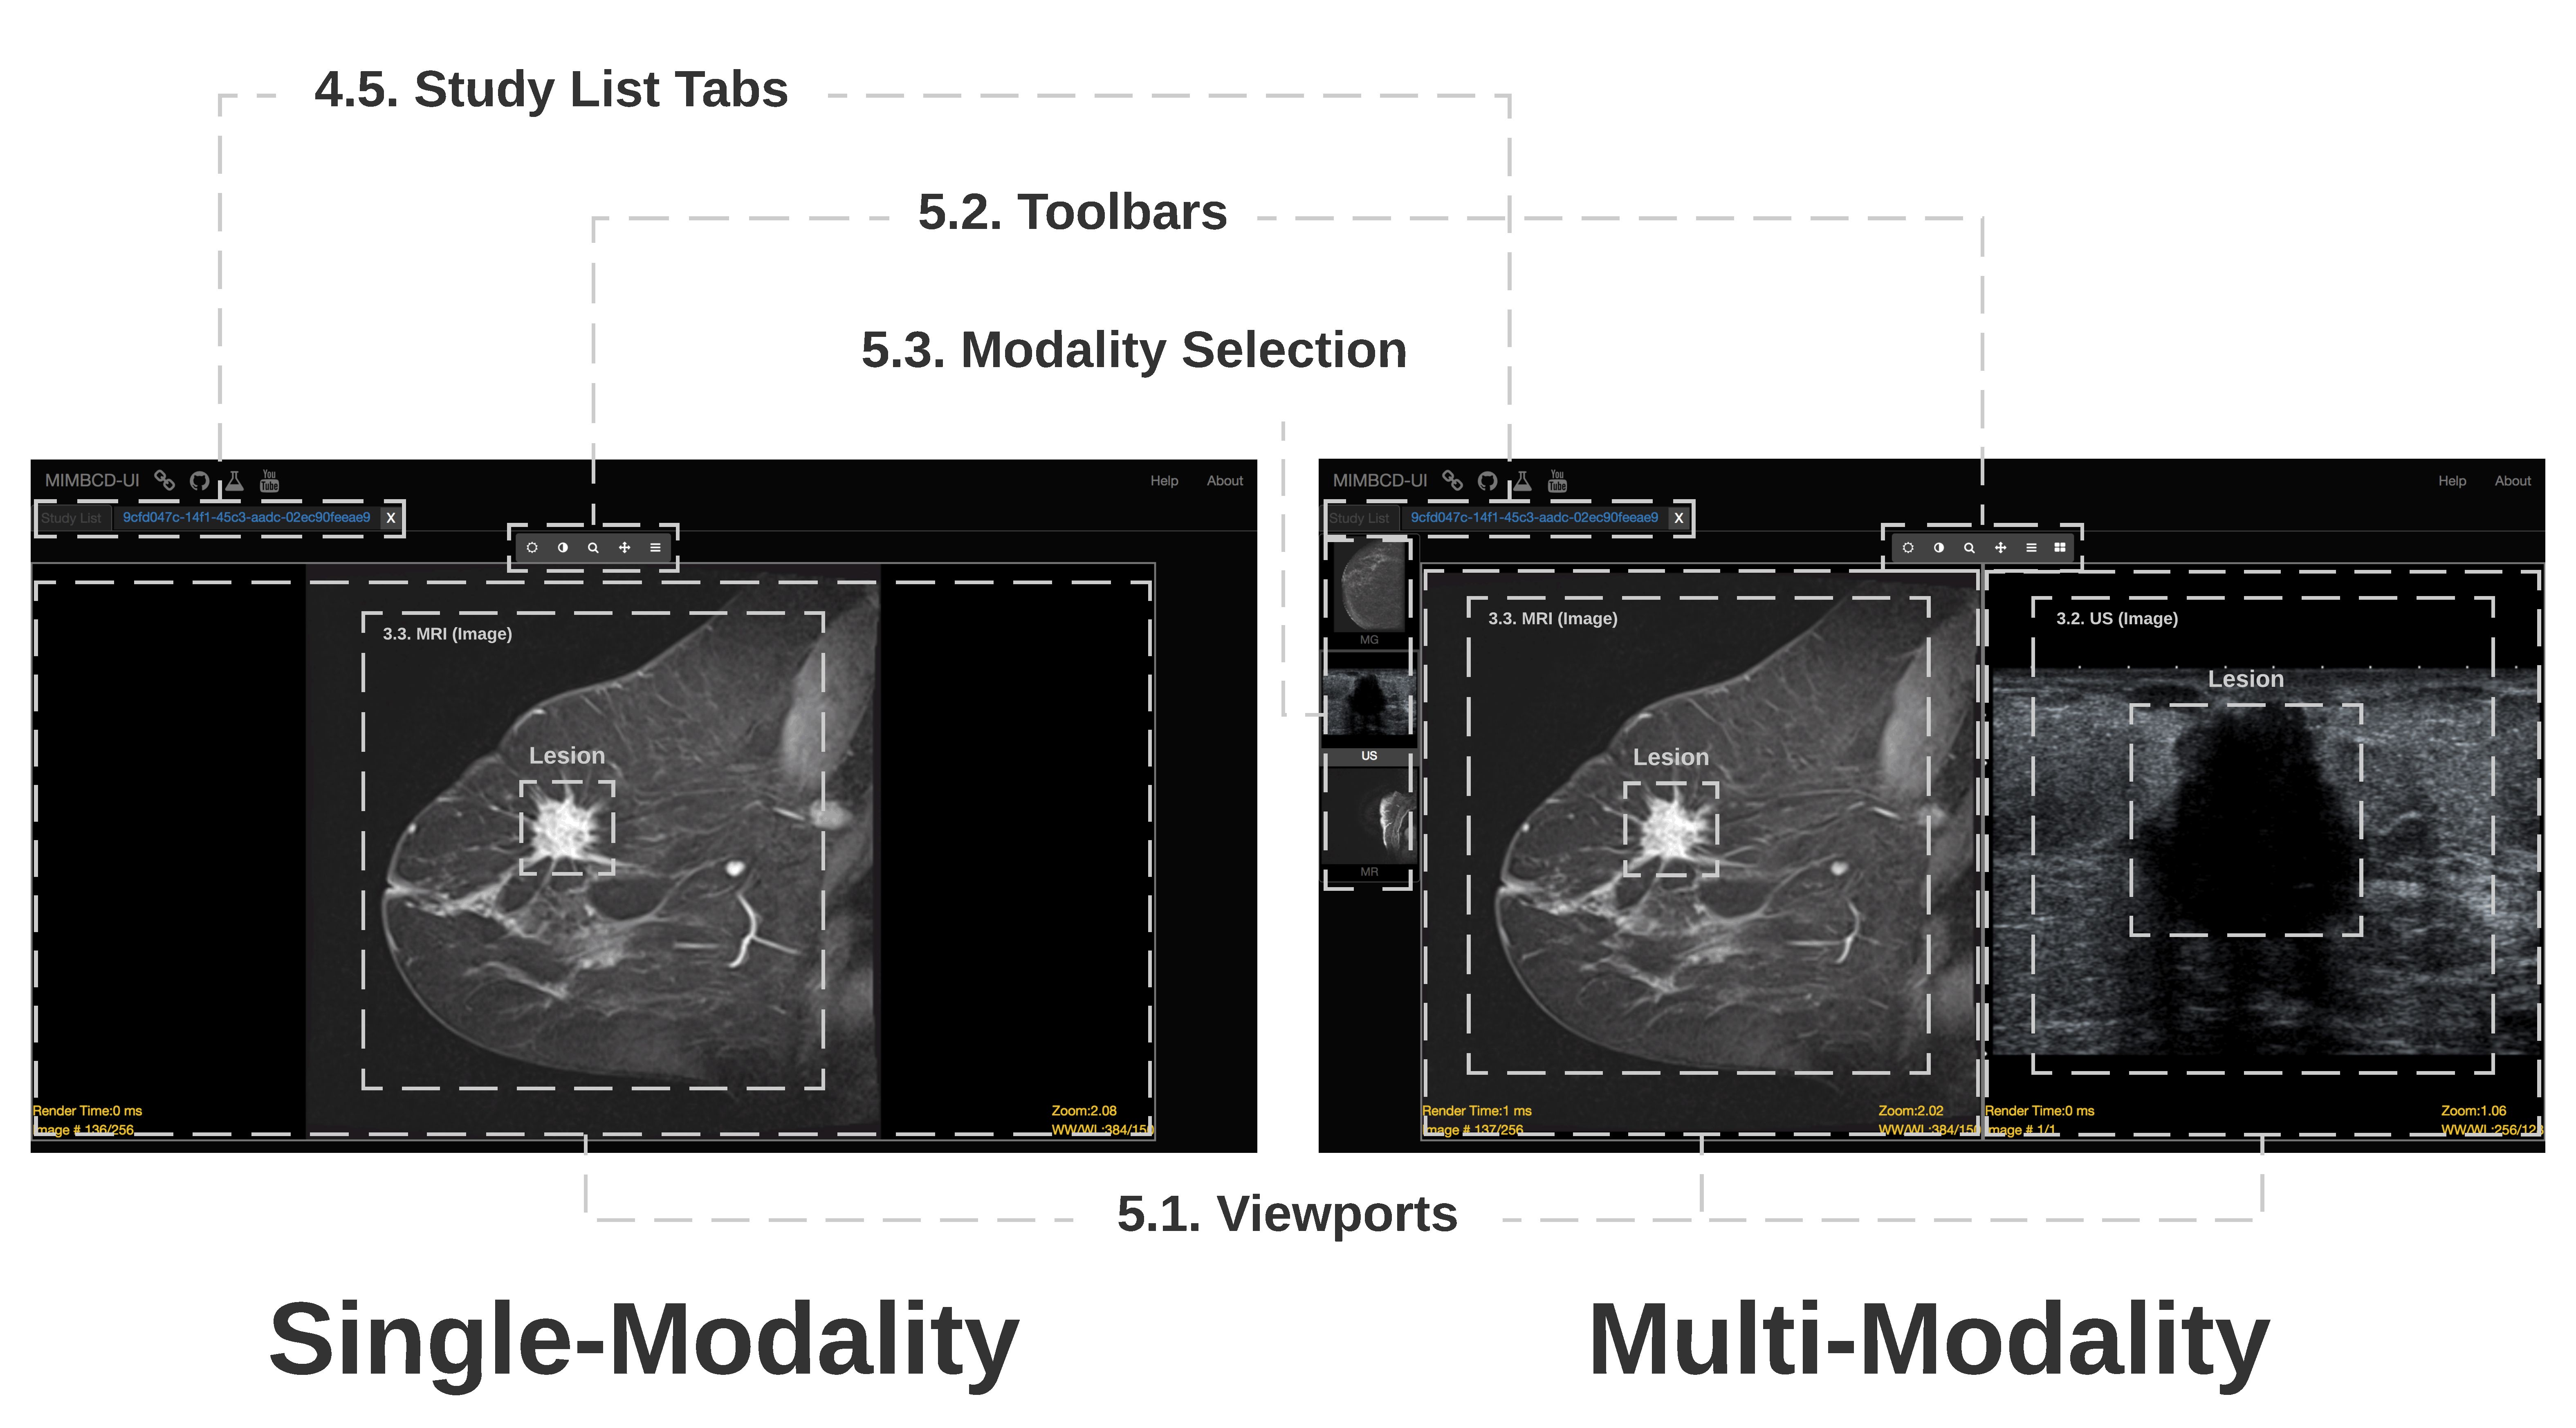
\includegraphics[width=\linewidth]{both_views}
\caption{\scriptsize \textit{Single-Modality} (left) and \textit{Multi-Modality} (right) Views. The UI components are as follows: \textit{4. List of Patient Views}; and \textit{4.5. Study List Tabs}; as well as \textit{5. Medical Imaging Diagnosis Views}; \textit{5.1. Viewports}; \textit{5.2. Toolbars}; and \textit{5.3. Modality Selection}.}
\label{fig:both_views}
\end{figure*}
%%%%%%%%%%%%%%%%%%%%%%%%%%%%%%%%%%%%%%%%%%%%%%%%%%%

\subsection{User Interface}

The User Interface (UI) consists of two main components:
\textit{4. List of Patient Views}; and
\textit{5. Medical Imaging Diagnosis Views}.
These two main components (Figure \ref{fig:both_views}) are also divided into several sections:
\textit{4.5. Study List Tabs};
\textit{5.1. Viewports};
\textit{5.2. Toolbars}; and
\textit{5.3. Modality Selection}.
Concerning \textit{5. Medical Imaging Diagnosis Views} ({\em Viewports}, {\em Toolbars} and {\em Modality Selection}) this contributes for the temporal awareness (\textit{TAS}).
More specifically, the clinician can probe for lesion patterns~\cite{10.1007/978-3-030-00928-1_62} via the \textit{5.1. Viewports}, processing the image by using the \textit{5.2. Toolbars} features (\textit{GTO}).
The system \textit{5.2. Toolbars} are supporting our image segmentation (\textit{ISS}).
The \textit{5.1. Viewports} are displayed right after the \textit{5.2. Toolbars}, designing around and for medical images (\textit{DMI}) what also improves the temporal awareness (\textit{TAS}) of the task.
On the same time, this design is supporting the way how to interact with several modalities (\textit{SMS}).
Regarding \textit{5.3. Modality Selection}, this allows to the clinician to find more different views (\textit{SMS}) of the same lesion, allowing to perform a better severity classification (Section \ref{sec:sec005}).
Finally, the clinician may look for the lesion shape and contour irregularities (Figure \ref{fig:both_views}) to focus on the segments of the image (\textit{ISS}).
After interacting with the system at the first time, the clinician is able to efficiently process (\textit{ISS}) several images at a same time and use the various given modalities (\textit{SMS}).

\subsection{Implementation}

\href{https://breastscreening.github.io/}{{\it BreastScreening}} was implemented using \href{https://cornerstonejs.org/}{{\it CornerstoneJS}}~\cite{urban2017lesiontracker} with a \href{https://nodejs.org/}{{\it NodeJS}} server.
To populate the system, we selected image sets from HFF patients and upload them into an \href{https://www.orthanc-server.com/}{{\it Orthanc}} server~\cite{Jodogne2018}.
Each patient has three modalities (MG, US and MRI).

The images were pre-processed and anonymized on the \href{https://www.orthanc-server.com/}{{\it Orthanc}} server and then consumed by the \href{https://breastscreening.github.io/}{{\it BreastScreening}} system.
The \href{https://breastscreening.github.io/}{{\it BreastScreening}} core is developed in \href{https://www.w3schools.com/js/}{{\it JavaScript}} with \href{https://www.w3schools.com/jquery/}{{\it jQuery}} for \href{https://www.w3schools.com/html/}{{\it HTML}} document manipulation, event handling and \href{https://github.com/cornerstonejs/dicomParser}{{\it dicomParser}} for parsing DICOM files.
The DICOM files can be loaded by drag-and-drop files into the browser window on the \href{https://www.orthanc-server.com/}{{\it Orthanc}} view.